\documentclass{labreport}

% UTF-8 support for Romanian diacritics in code listings
\lstset{style=python,
  literate={ă}{{\v{a}}}1
           {â}{{\^{a}}}1
           {î}{{\^{i}}}1
           {ș}{{\c{s}}}1
           {ț}{{\c{t}}}1
           {Ă}{{\v{A}}}1
           {Â}{{\^{A}}}1
           {Î}{{\^{I}}}1
           {Ș}{{\c{S}}}1
           {Ț}{{\c{T}}}1
}

\begin{document}

% ---------------------------------------------------------
% 1. TITLE PAGE
% ---------------------------------------------------------
\labtitle{3}{Polyalphabetic Ciphers: The Playfair Cipher for the Romanian Alphabet}{Ilie Covali}{gr. FAF-243}{asist. univ. Zaica Maia}

\tableofcontents
\newpage

% ---------------------------------------------------------
% 2. SHORT THEORY
% ---------------------------------------------------------
\section{Short Theory}

\subsection{Introduction to Polyalphabetic and Polygraphic Ciphers}
The historical evolution of classical cryptography was largely driven by the inherent vulnerability of monoalphabetic substitution ciphers: the direct preservation of the language's monographic frequency distribution. In simple monoalphabetic substitution, every distinct plaintext character maps deterministically to a fixed ciphertext character throughout the message. Consequently, single-letter frequency analysis, common digram counts, and pattern matching allow an analyst to reconstruct the plaintext and recover the key with modest computational effort.

To overcome this vulnerability, cryptographers developed two fundamental paradigms:
\begin{enumerate}
    \item \textbf{Polyalphabetic Substitution}: Varying the substitution alphabet dynamically as a function of character position. Introduced by Giovan Battista Bellaso in 1553 and later popularized by Blaise de Vigen\`{e}re in 1586, polyalphabetic ciphers shift characters according to a repeating key phrase, thereby combining multiple shift distributions and flattening the statistical frequency peaks of the plaintext.
    \item \textbf{Polygraphic (Digraphic) Substitution}: Encrypting units of multiple characters simultaneously rather than individual letters. Invented by Sir Charles Wheatstone in 1854 and championed for military adoption by Lord Lyon Playfair, the \textit{Playfair cipher} treats adjacent letter pairs (digraphs) as atomic encryption blocks. By mapping letter pairs to letter pairs, the cipher diffuses single-letter statistical properties: instead of 26 or 31 possible single-letter outcomes, the analyst must evaluate $26^2 = 676$ or $31^2 = 961$ possible digraph permutations.
\end{enumerate}

\subsection{Romanian Alphabet Adaptation: The \texorpdfstring{$6 \times 5$}{6x5} Grid Topology}
The standard classical Playfair cipher was originally designed for the 26-letter Latin alphabet. Because a $5 \times 5$ square matrix accommodates exactly 25 positions, classical English implementations merge \texttt{'I'} and \texttt{'J'} into a single cell ($J \to I$), consolidating the 26 letters into 25 discrete elements.

For this laboratory work, the task requires adapting the cipher for the Romanian alphabet comprising $N = 31$ letters:
\begin{equation}
\mathcal{A}_{\text{ro}} = [\text{A, Ă, Â, B, C, D, E, F, G, H, I, Î, J, K, L, M, N, O, P, Q, R, S, Ș, T, Ț, U, V, W, X, Y, Z}]
\end{equation}

As specified in the laboratory guidelines, when the target alphabet does not form a perfect square, rectangular matrices ($6 \times 5$, $5 \times 6$, etc.) are adopted, and low-frequency or interchangeable letters are consolidated. In the Romanian language, the letter \texttt{'J'} occurs with low frequency in core vocabulary and is phonetically and orthographically close to \texttt{'I'}. Merging \texttt{'J'} into \texttt{'I'} ($J \to I$) reduces the 31 letters to exactly 30 unique symbols:
\begin{equation}
\begin{split}
\mathcal{A}_{\text{playfair}} = [&\text{A, Ă, Â, B, C, D, E, F, G, H, I, Î, K, L, M,} \\
&\text{N, O, P, Q, R, S, Ș, T, Ț, U, V, W, X, Y, Z}]
\end{split}
\end{equation}
Because $|\mathcal{A}_{\text{playfair}}| = 30 = 6 \times 5$, all 30 letters populate a rectangular matrix of $R = 6$ rows and $C = 5$ columns without leaving vacant cells.

\subsection{Mathematical Model of the \texorpdfstring{$6 \times 5$}{6x5} Playfair Cipher}
Let $\mathcal{M}$ denote the $6 \times 5$ matrix represented as a bijection:
\begin{equation}
\Phi: \mathbb{Z}_6 \times \mathbb{Z}_5 \to \mathcal{A}_{\text{playfair}}, \quad (r, c) \mapsto \mathcal{M}[r][c]
\end{equation}
with inverse coordinate lookup $\Phi^{-1}: \mathcal{A}_{\text{playfair}} \to \mathbb{Z}_6 \times \mathbb{Z}_5$, such that $\Phi^{-1}(\alpha) = (r_\alpha, c_\alpha)$.

\subsubsection{Digraph Formation and Collision Resolution}
A plaintext message $M$ of length $|M|$ is first stripped of whitespace and non-alphabet characters, with all letters converted to uppercase and any occurrence of \texttt{'J'} mapped to \texttt{'I'}. The string is then partitioned into consecutive digraphs $(P_1, P_2)$:
\begin{enumerate}
    \item \textbf{Collision Rule}: If $P_1 = P_2$ within an active pair, a null separator character is inserted between them. The primary filler character is \texttt{'X'} (or \texttt{'Z'} if $P_1 = \texttt{'X'}$), deferring $P_2$ to initiate the subsequent digraph.
    \item \textbf{Odd-Length Padding}: If an isolated character remains at the end of the text, an additional filler character (\texttt{'X'}, or \texttt{'Z'} if the terminal letter is \texttt{'X'}) is appended to ensure an even number of symbols.
\end{enumerate}

\subsubsection{Encryption Rules}
For each prepared digraph $(P_1, P_2)$ with matrix coordinates $(r_1, c_1) = \Phi^{-1}(P_1)$ and $(r_2, c_2) = \Phi^{-1}(P_2)$, the ciphertext pair $(C_1, C_2) = E(P_1, P_2)$ is defined as:
\begin{equation}
(C_1, C_2) =
\begin{cases}
\big(\Phi(r_1, (c_1 + 1) \bmod 5), \, \Phi(r_2, (c_2 + 1) \bmod 5)\big), & \text{if } r_1 = r_2 \text{ (Same Row)} \\[6pt]
\big(\Phi((r_1 + 1) \bmod 6, c_1), \, \Phi((r_2 + 1) \bmod 6, c_2)\big), & \text{if } c_1 = c_2 \text{ (Same Column)} \\[6pt]
\big(\Phi(r_1, c_2), \, \Phi(r_2, c_1)\big), & \text{otherwise (Rectangle Rule)}
\end{cases}
\end{equation}

\subsubsection{Decryption Rules}
Decryption performs the exact inverse transformation on each ciphertext digraph $(C_1, C_2)$ with coordinates $(r_1, c_1) = \Phi^{-1}(C_1)$ and $(r_2, c_2) = \Phi^{-1}(C_2)$:
\begin{equation}
(P_1, P_2) = D(C_1, C_2) =
\begin{cases}
\big(\Phi(r_1, (c_1 - 1) \bmod 5), \, \Phi(r_2, (c_2 - 1) \bmod 5)\big), & \text{if } r_1 = r_2 \text{ (Same Row)} \\[6pt]
\big(\Phi((r_1 - 1) \bmod 6, c_1), \, \Phi((r_2 - 1) \bmod 6, c_2)\big), & \text{if } c_1 = c_2 \text{ (Same Column)} \\[6pt]
\big(\Phi(r_1, c_2), \, \Phi(r_2, c_1)\big), & \text{otherwise (Rectangle Rule)}
\end{cases}
\end{equation}

\subsubsection{Proof of Invertibility}
We verify that $D(E(P_1, P_2)) = (P_1, P_2)$ across all three geometric cases:
\begin{itemize}
    \item \textbf{Case 1 (Same Row, $r_1 = r_2$):}
    \begin{align}
    c_i' &= (c_i + 1) \bmod 5 \notag \\
    c_i'' &= (c_i' - 1) \bmod 5 = ((c_i + 1 \bmod 5) - 1) \bmod 5 = c_i \bmod 5 = c_i
    \end{align}
    Since the row index $r_i$ remains unchanged, $\Phi(r_i, c_i'') = \Phi(r_i, c_i) = P_i$.
    \item \textbf{Case 2 (Same Column, $c_1 = c_2$):}
    \begin{align}
    r_i' &= (r_i + 1) \bmod 6 \notag \\
    r_i'' &= (r_i' - 1) \bmod 6 = ((r_i + 1 \bmod 6) - 1) \bmod 6 = r_i \bmod 6 = r_i
    \end{align}
    Since the column index $c_i$ remains unchanged, $\Phi(r_i'', c_i) = \Phi(r_i, c_i) = P_i$.
    \item \textbf{Case 3 (Rectangle Rule, $r_1 \ne r_2$ and $c_1 \ne c_2$):}
    Encryption produces $C_1 = \Phi(r_1, c_2)$ and $C_2 = \Phi(r_2, c_1)$. Applying the rectangle rule on $(C_1, C_2)$ yields:
    \begin{equation}
    P_1' = \Phi(r_1, c_{C_2}) = \Phi(r_1, c_1) = P_1, \quad P_2' = \Phi(r_2, c_{C_1}) = \Phi(r_2, c_2) = P_2
    \end{equation}
\end{itemize}
Thus, the transformation is bijective, deterministic, and strictly lossless.

\subsection{Key Space and Cryptanalytic Complexity}
The theoretical total number of distinct matrix configurations over 30 unique symbols is:
\begin{equation}
N_{\text{total}} = 30! \approx 2.6525 \times 10^{32}
\end{equation}
However, multiple matrices yield identical digraph substitution mappings due to rotational symmetries. In a $6 \times 5$ grid, cyclically shifting all rows preserves vertical relative offsets, and cyclically shifting all columns preserves horizontal relative offsets. There are $6$ row shift equivalences and $5$ column shift equivalences, yielding $6 \times 5 = 30$ symmetrically equivalent keys for any given matrix.

When the matrix is constructed from a secret keyword $K$ of length $\ge 7$, the actual keyspace corresponds to the number of unique character sequences of length $m$ drawn from 30 letters, followed by deterministic alphabetical completion. For a minimal keyword of 7 distinct characters, the partial permutation count is:
\begin{equation}
P(30, 7) = \frac{30!}{(30-7)!} = \frac{30!}{23!} = 30 \times 29 \times 28 \times 27 \times 26 \times 25 \times 24 = 10,260,432,000 \approx 1.03 \times 10^{10}
\end{equation}
For longer keywords ($m \ge 12$), the keyspace exceeds $10^{16}$ combinations, rendering brute-force exhaustive search computationally prohibitive without specialized parallel architectures.

\newpage

% ---------------------------------------------------------
% 3. IMPLEMENTATION
% ---------------------------------------------------------
\section{Implementation}

The complete cryptosystem is implemented in Python 3 within the module \texttt{playfair.py}. It follows defensive programming principles, ensuring thorough input sanitization, clear error reporting, and transparent 2D matrix visualization.

\subsection{Alphabet Definitions and Diacritic Normalization}
The Romanian alphabet contains five characters with diacritical marks (\texttt{ă}, \texttt{â}, \texttt{î}, \texttt{ș}, \texttt{ț}). To prevent character encoding inconsistencies across different platforms and keyboard layouts, legacy cedilla variants (\texttt{ş}, \texttt{ţ}) are normalized to standard Romanian comma-below characters (\texttt{ș}, \texttt{ț}):

\begin{lstlisting}[style=python]
ROMANIAN_ALPHABET = [
    "A", "Ă", "Â", "B", "C", "D", "E", "F", "G", "H", "I", "Î", "J", "K",
    "L", "M", "N", "O", "P", "Q", "R", "S", "Ș", "T", "Ț", "U", "V", "W",
    "X", "Y", "Z"
]

PLAYFAIR_ALPHABET = [
    "A", "Ă", "Â", "B", "C", "D", "E", "F", "G", "H", "I", "Î", "K",
    "L", "M", "N", "O", "P", "Q", "R", "S", "Ș", "T", "Ț", "U", "V", "W",
    "X", "Y", "Z"
]
MATRIX_ROWS = 6
MATRIX_COLS = 5
\end{lstlisting}
\textit{Comment:} \texttt{PLAYFAIR\_ALPHABET} contains exactly 30 characters, perfectly filling the $6 \times 5$ matrix after merging $J \to I$.

\subsection{Input Validation}
Input validation adheres strictly to the constraints outlined in Task 3.1:
\begin{enumerate}
    \item \textbf{Keyword Length}: Must contain at least 7 characters.
    \item \textbf{Character Set}: Only valid Romanian alphabet letters are accepted. If unsupported characters (digits, symbols, punctuation) are entered, the program halts and informs the user of the allowed character range.
\end{enumerate}

\begin{lstlisting}[style=python]
def validate_keyword(keyword: str) -> bool:
    if not keyword:
        print("Error: Keyword cannot be empty.")
        return False
    clean_key = keyword.strip()
    if len(clean_key) < 7:
        print(f"Error: Keyword is too short ({len(clean_key)} chars)! It must be at least 7 characters long.")
        return False
    for char in clean_key:
        norm = normalize_character(char)
        if norm not in ROMANIAN_ALPHABET and norm != " ":
            print(f"Error: Invalid character '{char}' in keyword!")
            print("Allowed characters: A-Z, Ă, Â, Î, Ș, Ț (letters only, min length 7).")
            return False
    return True

def validate_text(text: str) -> bool:
    if not text or not text.strip():
        print("Error: Input text cannot be empty.")
        return False
    for char in text:
        norm = normalize_character(char)
        if norm not in ROMANIAN_ALPHABET and norm != " ":
            print(f"Error: Invalid character '{char}' detected!")
            print("Allowed characters: letters from Romanian alphabet (A-Z, a-z, ă, â, î, ș, ț) and spaces.")
            return False
    return True
\end{lstlisting}

\subsection{Matrix Generation}
The $6 \times 5$ matrix is constructed dynamically from the keyword by deduplicating characters in their order of first appearance and appending unused letters of $\mathcal{A}_{\text{playfair}}$:

\begin{lstlisting}[style=python]
def build_matrix(keyword: str):
    unique_key = []
    for char in keyword:
        norm = normalize_character(char)
        if norm == " ":
            continue
        c = "I" if norm == "J" else norm
        if c in PLAYFAIR_ALPHABET and c not in unique_key:
            unique_key.append(c)

    for char in PLAYFAIR_ALPHABET:
        if char not in unique_key:
            unique_key.append(char)

    matrix = [unique_key[i:i + MATRIX_COLS] for i in range(0, len(unique_key), MATRIX_COLS)]

#    matrix = []
#    for i in range(0, len(unique_key), MATRIX_COLS):
#        row = unique_key[i:i + MATRIX_COLS]
#        matrix.append(row)
    return matrix
\end{lstlisting}

\subsection{Digraph Formulation}
Plaintext letters are paired iteratively. When adjacent identical characters are detected within a pair, a filler character is inserted:

\begin{lstlisting}[style=python]
def prepare_plaintext(text: str):
    clean = []
    for char in text:
        norm = normalize_character(char)
        if norm == " ":
            continue
        c = "I" if norm == "J" else norm
        if c in PLAYFAIR_ALPHABET:
            clean.append(c)

    pairs = []
    i = 0
    n = len(clean)
    while i < n:
        first = clean[i]
        if i + 1 < n:
            second = clean[i + 1]
            if first == second:
                filler = "Z" if first == "X" else "X"
                pairs.append((first, filler))
                i += 1
            else:
                pairs.append((first, second))
                i += 2
        else:
            filler = "Z" if first == "X" else "X"
            pairs.append((first, filler))
            i += 1
    return pairs
\end{lstlisting}

\subsection{Core Cryptographic Transformation}
The substitution logic implements modular arithmetic across rows ($c \pm 1 \pmod 5$) and columns ($r \pm 1 \pmod 6$):

\begin{lstlisting}[style=python]
def encrypt_pair(matrix, pos, p1: str, p2: str):
    r1, c1 = pos[p1]
    r2, c2 = pos[p2]
    if r1 == r2:
        return matrix[r1][(c1 + 1) % MATRIX_COLS] + matrix[r2][(c2 + 1) % MATRIX_COLS]
    elif c1 == c2:
        return matrix[(r1 + 1) % MATRIX_ROWS][c1] + matrix[(r2 + 1) % MATRIX_ROWS][c2]
    else:
        return matrix[r1][c2] + matrix[r2][c1]

def decrypt_pair(matrix, pos, c1: str, c2: str):
    r1, col1 = pos[c1]
    r2, col2 = pos[c2]
    if r1 == r2:
        return matrix[r1][(col1 - 1) % MATRIX_COLS] + matrix[r2][(col2 - 1) % MATRIX_COLS]
    elif col1 == col2:
        return matrix[(r1 - 1) % MATRIX_ROWS][col1] + matrix[(r2 - 1) % MATRIX_ROWS][col2]
    else:
        return matrix[r1][col2] + matrix[r2][col1]
\end{lstlisting}

\newpage

% ---------------------------------------------------------
% 4. RESULTS
% ---------------------------------------------------------
\section{Results}

This section documents actual program execution across Romanian and standard test samples, demonstrating encryption, decryption, matrix generation, and input validation handling.

\subsection{Demonstration 1: Romanian Text Encryption with Diacritics}
Figure~\ref{fig:enc_ro} shows the encryption of the Romanian phrase containing diacritics:
\begin{center}
\texttt{"cifruri polialfabetice și securitatea datelor"}
\end{center}
using the secret keyword \texttt{"universitate"}. The program constructs the $6 \times 5$ matrix, prints the partitioned digraphs, and outputs the resulting ciphertext:
\begin{center}
\texttt{"ÎTÂĂRÂTXȘHVTȘLSDIĂTÎĂZNTIFRÂTCĂAVĂKDĂIHȘTȚ"}
\end{center}

\begin{figure}[H]
    \centering
    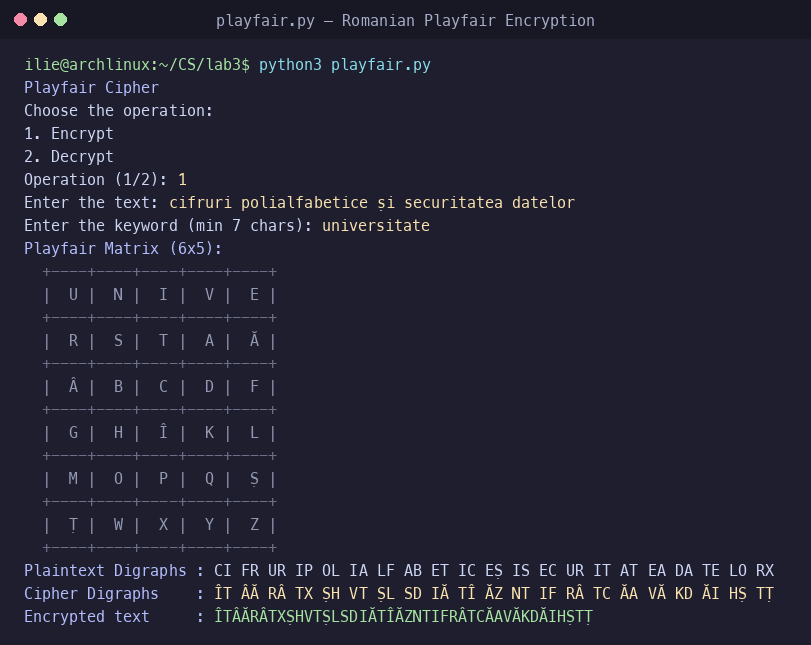
\includegraphics[width=0.92\textwidth]{images/playfair_encrypt_ro.png}
    \caption{Encryption of Romanian plaintext with diacritics on $6 \times 5$ matrix ($K = \text{"universitate"}$).}
    \label{fig:enc_ro}
\end{figure}

\subsection{Demonstration 2: Romanian Text Decryption}
Figure~\ref{fig:dec_ro} demonstrates the exact reverse operation. Decrypting the ciphertext with the same keyword recovers the character stream \texttt{"CIFRURIPOLIALFABETICEȘISECURITATEADATELORX"}, which restores the original message \texttt{"cifruri polialfabetice și securitatea datelor"} (with trailing padding letter \texttt{'X'} trimmed).

\begin{figure}[H]
    \centering
    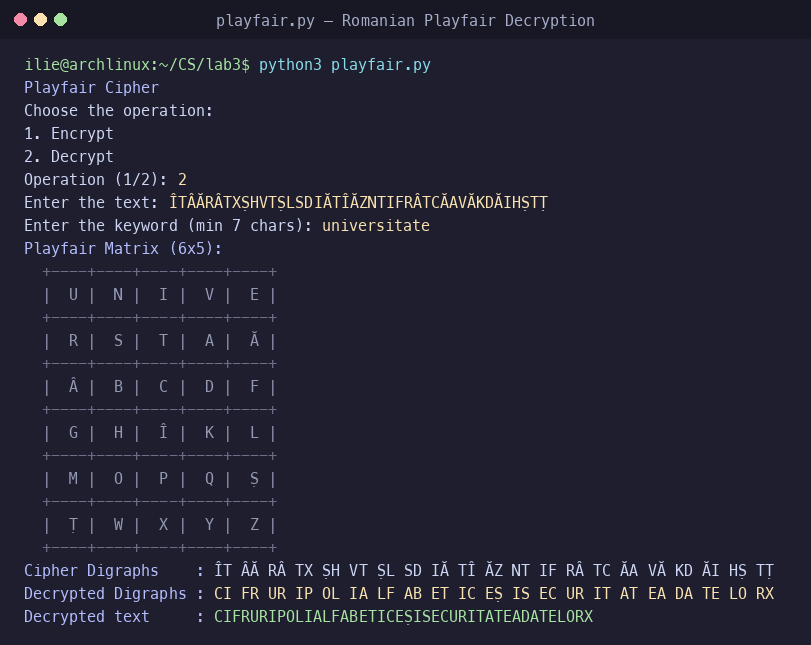
\includegraphics[width=0.92\textwidth]{images/playfair_decrypt_ro.png}
    \caption{Decryption of Romanian ciphertext on $6 \times 5$ matrix ($K = \text{"universitate"}$).}
    \label{fig:dec_ro}
\end{figure}

\newpage
\subsection{Demonstration 3: Standard Cryptographic Sample Execution}
Figures~\ref{fig:enc_en} and~\ref{fig:dec_en} illustrate encryption and decryption of the message \texttt{"securitatea informatiei"} using keyword \texttt{"criptografie"}. The ciphertext produced is \texttt{"UGTQIPIEEHBAMEGCLFCPAT"}, which is then completely decrypted back to its original character sequence.

\begin{figure}[H]
    \centering
    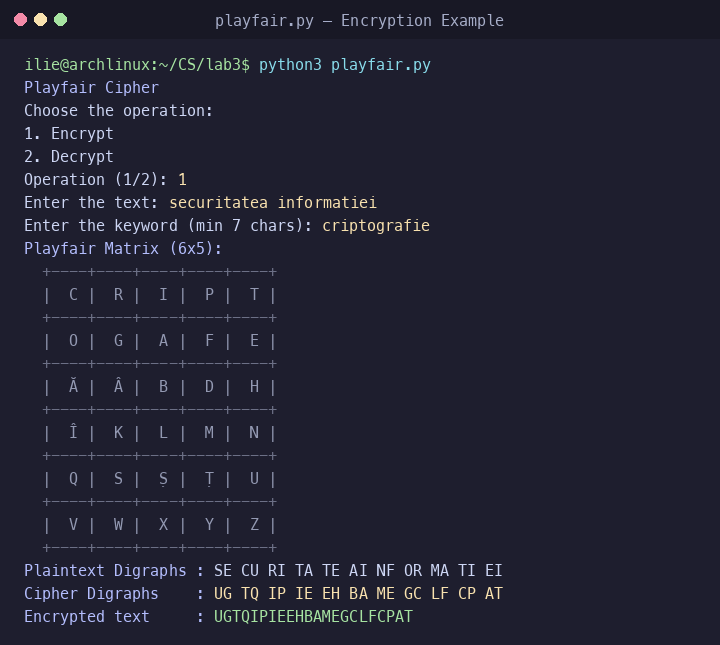
\includegraphics[width=0.92\textwidth]{images/playfair_encrypt_en.png}
    \caption{Playfair encryption execution for \texttt{"securitatea informatiei"} ($K = \text{"criptografie"}$).}
    \label{fig:enc_en}
\end{figure}

\begin{figure}[H]
    \centering
    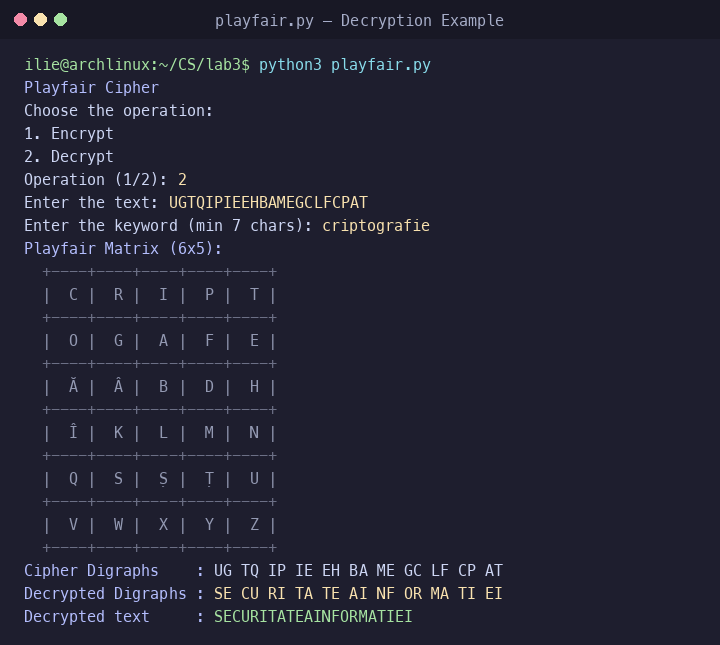
\includegraphics[width=0.92\textwidth]{images/playfair_decrypt_en.png}
    \caption{Playfair decryption execution for \texttt{"securitatea informatiei"}.}
    \label{fig:dec_en}
\end{figure}

\newpage
\subsection{Demonstration 4: Defensive Input Validation}

\subsubsection{Keyword Too Short \texorpdfstring{($\text{length} < 7$)}{(length < 7)}}
Figure~\ref{fig:val_key} illustrates the defensive rejection of a short keyword (\texttt{"cheie"}, length 5). The program detects that the length is below the required 7 characters and halts execution safely with an informative error message.

\begin{figure}[H]
    \centering
    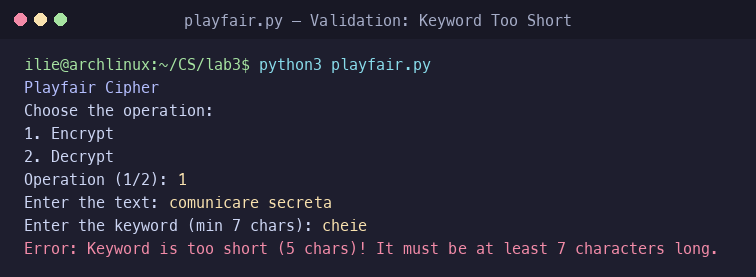
\includegraphics[width=0.92\textwidth]{images/playfair_invalid_key_short.png}
    \caption{Input validation: Rejection of keyword shorter than 7 characters.}
    \label{fig:val_key}
\end{figure}

\subsubsection{Invalid Characters and Range Suggestion}
Figure~\ref{fig:val_char} depicts the detection of illegal characters (underscores, digits, and punctuation in \texttt{"parola\_secreta\#2026!"}). The program alerts the user to the offending character and explicitly specifies the allowed character diapason.

\begin{figure}[H]
    \centering
    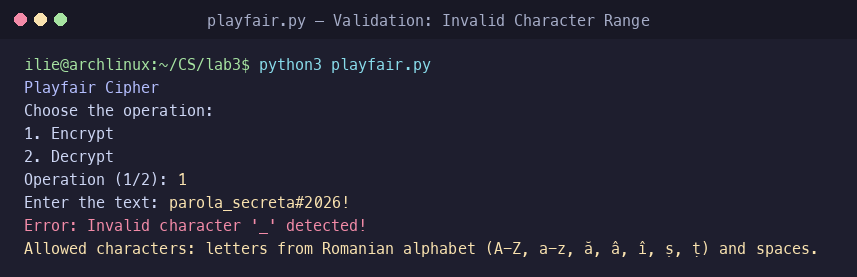
\includegraphics[width=0.92\textwidth]{images/playfair_invalid_char.png}
    \caption{Input validation: Offending character detection and allowed range suggestion.}
    \label{fig:val_char}
\end{figure}

\subsubsection{Invalid Operation Choice}
Figure~\ref{fig:val_op} displays the handling of an invalid operation selection (e.g. entering \texttt{5} instead of \texttt{1} or \texttt{2}).

\begin{figure}[H]
    \centering
    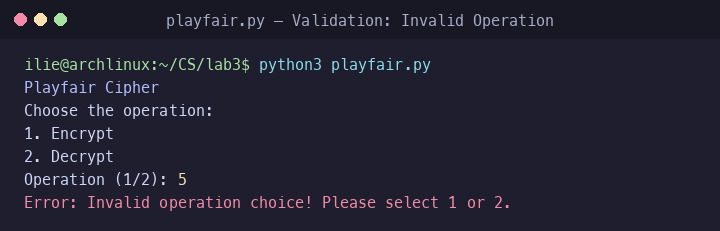
\includegraphics[width=0.92\textwidth]{images/playfair_invalid_op.png}
    \caption{Input validation: Rejection of invalid menu operation choice.}
    \label{fig:val_op}
\end{figure}

\newpage

% ---------------------------------------------------------
% 5. CONCLUSIONS
% ---------------------------------------------------------
\section{Conclusions}

Through the implementation, mathematical formalization, and testing of the Playfair cipher adapted for the Romanian alphabet, the following conclusions are established:

\begin{enumerate}
    \item \textbf{Diffusion of Monographic Statistics:} The Playfair cipher represents a major conceptual advance over classical monoalphabetic substitution ciphers (such as standard and permuted Caesar). By operating on digraphs rather than individual characters, single-letter frequency distributions are thoroughly obscured. A single plaintext letter maps to multiple different ciphertext letters depending on its paired counterpart, directly impeding classical monographic frequency cryptanalysis.
    
    \item \textbf{Geometrical Flexibility of Rectangular Grids:} While the classical Playfair algorithm relies on a square $5 \times 5$ matrix for 25 Latin letters, this laboratory work proved that the underlying geometric substitution rules (same row, same column, rectangle) extend naturally to rectangular matrices of dimension $R \times C$. For the Romanian language ($N = 31$), merging $J \to I$ provides exactly 30 unique symbols that map onto a $6 \times 5$ grid without leaving unused cells. The modular arithmetic shifts $(c \pm 1 \bmod 5)$ and $(r \pm 1 \bmod 6)$ maintain bijection and invertibility.
    
    \item \textbf{Residual Vulnerabilities of Digraphic Ciphers:} Despite its superiority over Caesar ciphers, Playfair is not unconditionally secure. Because digraphs are treated as atomic units, digraph frequency distributions remain partially preserved. In Romanian, common digraphs such as \texttt{"DE"}, \texttt{"RE"}, and \texttt{"IN"} appear with predictable frequencies. Furthermore, the rectangle rule creates symmetrical pairs (e.g. if $E(AB) = CD$, then $E(BA) = DC$), and the cipher never encrypts a letter to itself. Modern cryptanalysts using simulated annealing, genetic algorithms, or hill climbing can reconstruct the matrix from ciphertexts of a few hundred words.
    
    \item \textbf{Deterministic Nature of Known-Key Decryption:} Unlike automated cryptanalysis of Vigen\`{e}re or Playfair without a key (which generates vast hypothesis spaces requiring language scoring to detect legitimate plaintexts), symmetric decryption with the known secret key is completely deterministic. It yields exactly one unique plaintext character stream, leaving only the standard manual restoration of sentence whitespace as specified by the laboratory guidelines.
\end{enumerate}

% ---------------------------------------------------------
% 6. SOURCE CODE
% ---------------------------------------------------------
\section{Source Code}

The complete source code for this laboratory work is version-controlled and hosted on GitHub:

\begin{center}
\textbf{GitHub Repository Link:}\\
\url{https://github.com/owhowh0/cs-labs/tree/main/lab3}
\end{center}

\subsection{Project Repository Structure}
\begin{itemize}
    \item \texttt{playfair.py}: Core implementation of the Romanian $6 \times 5$ Playfair cipher, defensive validation, and interactive CLI.
    \item \texttt{generate\_screenshots.py}: Automation script rendering terminal execution figures.
    \item \texttt{report/}:
    \begin{itemize}
        \item \texttt{report.tex}: The complete \LaTeX{} source code for this report.
        \item \texttt{report.pdf}: Compiled PDF report.
        \item \texttt{labreport.cls}: Custom university report document class.
        \item \texttt{titlesec.sty}: Heading formatting package.
        \item \texttt{images/}: High-resolution terminal execution captures.
    \end{itemize}
    \item \texttt{pyproject.toml}: Project dependencies and execution metadata managed with \texttt{uv}.
    \item \texttt{README.md}: Technical documentation and execution guide.
\end{itemize}

\end{document}
